\section{Conditional probabilities, random variables and the binomial distribution}

\subsection{Conditional Probability}
\begin{defn}[\textbf{Conditional Probability}]
Let $A, B \subseteq \Omega$ be events with $\PP(A) \not=0$ The conditional probability of $B$ given $A$ is defined by
\[\PP(B \vert A) := \frac{\PP(A \cap B)}{\PP(A)}.\]
\end{defn}
\noindent Here, $\PP( B \vert A)=$"The probability of $B$ occurring when we know that $A$ has occurred.". This equation is often used ``multiplied out'' as
\[\PP(A \cap B) = \PP(B) \, \PP(A \st B). \]
This makes it clearer that the meaning of $\PP(A \st B)$ is that it is \emph{the probability of $A$ given that we know that $B$ has occurred.}
\begin{example}
I roll two D6 in secret. I have a look and reveal to you that the sum of the two dice is $8$. What is the probability that one of the dice shows a '$6$'?\\ \linebreak
Let $\Omega = \{ (\omega_1,\omega_2):\ \omega_1,\omega_2 \in \{1, \ldots, 6 \}\}$ and $\PP(\{\omega\}) = \frac{1}{36}$. Define 
\[A:=\{ (\omega_1,\omega_2): \omega_1+ \omega_2 = 8 \} = \{ (2,6),(3,5), (4,4), (5,3), (6,2)\}\]
and 
\[B:=\{ (6,1),\ldots,(6,5),(6,6),(5,6),\ldots,(1,6).\]
\linebreak\noindent Then $\vert A \vert =5$, $A \cap B= \{ (2,6),(6,2)\}$ and hence $\vert A \cap B \vert = 2$ giving us that
\[ \PP(B \vert A) = \frac{\PP(A \cap B)}{\PP(A)} = \frac{ 2/36}{5/36} = \frac25.\]
\end{example}

\begin{prop}[\textbf{Law of Total Probability}]
Let $n\in \NN$ and $A_i$ for all $i \in \{1,\ldots,n\}$ be disjoint events that partition the state space $\Omega$. For an arbitrary event $B$ we have
\begin{align*}
\PP(B)
= \sum_{i=1}^n \PP(B \vert A_i ) \PP(A_i).
\end{align*}
\end{prop}
\begin{corr}
For two events $A$ and $B$ it holds true that
\begin{align*}
\PP(B) = \PP(B \vert A) \PP(A) + \PP(B \vert A^C) \PP(A^C)
.
\end{align*}
\end{corr}
\begin{proof}
We will consider just the case $n=2$; the general case is similar. Thus we partition the sample space into a disjoint union $S = A \cup A^c$.  Then also $B$ is partitioned as 
 \[
    B = ( B \cap A ) \cup (B \cap A^c) 
 \]
So 
 \begin{eqnarray*}
    \PP(B) & =& \PP( B \cap A ) \cup \PP (B \cap A^c) \\ 
     &=& \PP(B \st A) \, \PP(A) + \PP(B \st A^c) \, \PP(A^c)
 \end{eqnarray*} 
\end{proof}
\subsection{Bayes' Theorem} 

Bayes' Theorem (or sometimes Bayes' ``rule'' or ``formula'') has a simple proof but is of huge importance in  answering questions about how probable it is that some event has ``caused'' an observed result.  It is hugely important in Statistics: there is a whole approach to statistical analysis using ``Bayesian methods''.  It is fundamental also in machine learning. 

\begin{center}
    PUT IN SOME CLEVER LINKING PASSAGE HERE
\end{center}
I toss a coin 5 times and obtain 3 or more heads.  What is the probability that the first toss was H? 

Let $B$ be the event of 3 or more H out of 5.  Then by binomial 
 \[
     \PP( B) = \frac1{2^5}\left(  \binom53 + \binom54 + \binom55 \right)   =  \frac{16}{2^5}.
 \]
Let $A$ be the event that the first toss is H.  Then $A \cap B$ is the event of tossing a H, followed by at least 2 H in the remaining 4 tosses. So by binomial again 
 \[
   \PP(A \cap B) = \frac12 \; \frac1{2^4} \left(  \binom42 + \binom43 +\binom 44\right) = \frac{11}{2^5}.
 \]
 So dividing, 
  \[
  \PP(A \st B) = \frac{11/2^5}{16/2^5} = \frac{11}{16}.  
 \]

In taking probabilities conditional upon an event $B$, one is zooming in on $B$, replacing ones initial sample space $S$ with $B$. In doing so, one becomes interested in $A \cap B$ rather than $A$ itself.  Figure~\ref{condo} illustrates what is going on. 

\begin{figure}[h] \centering
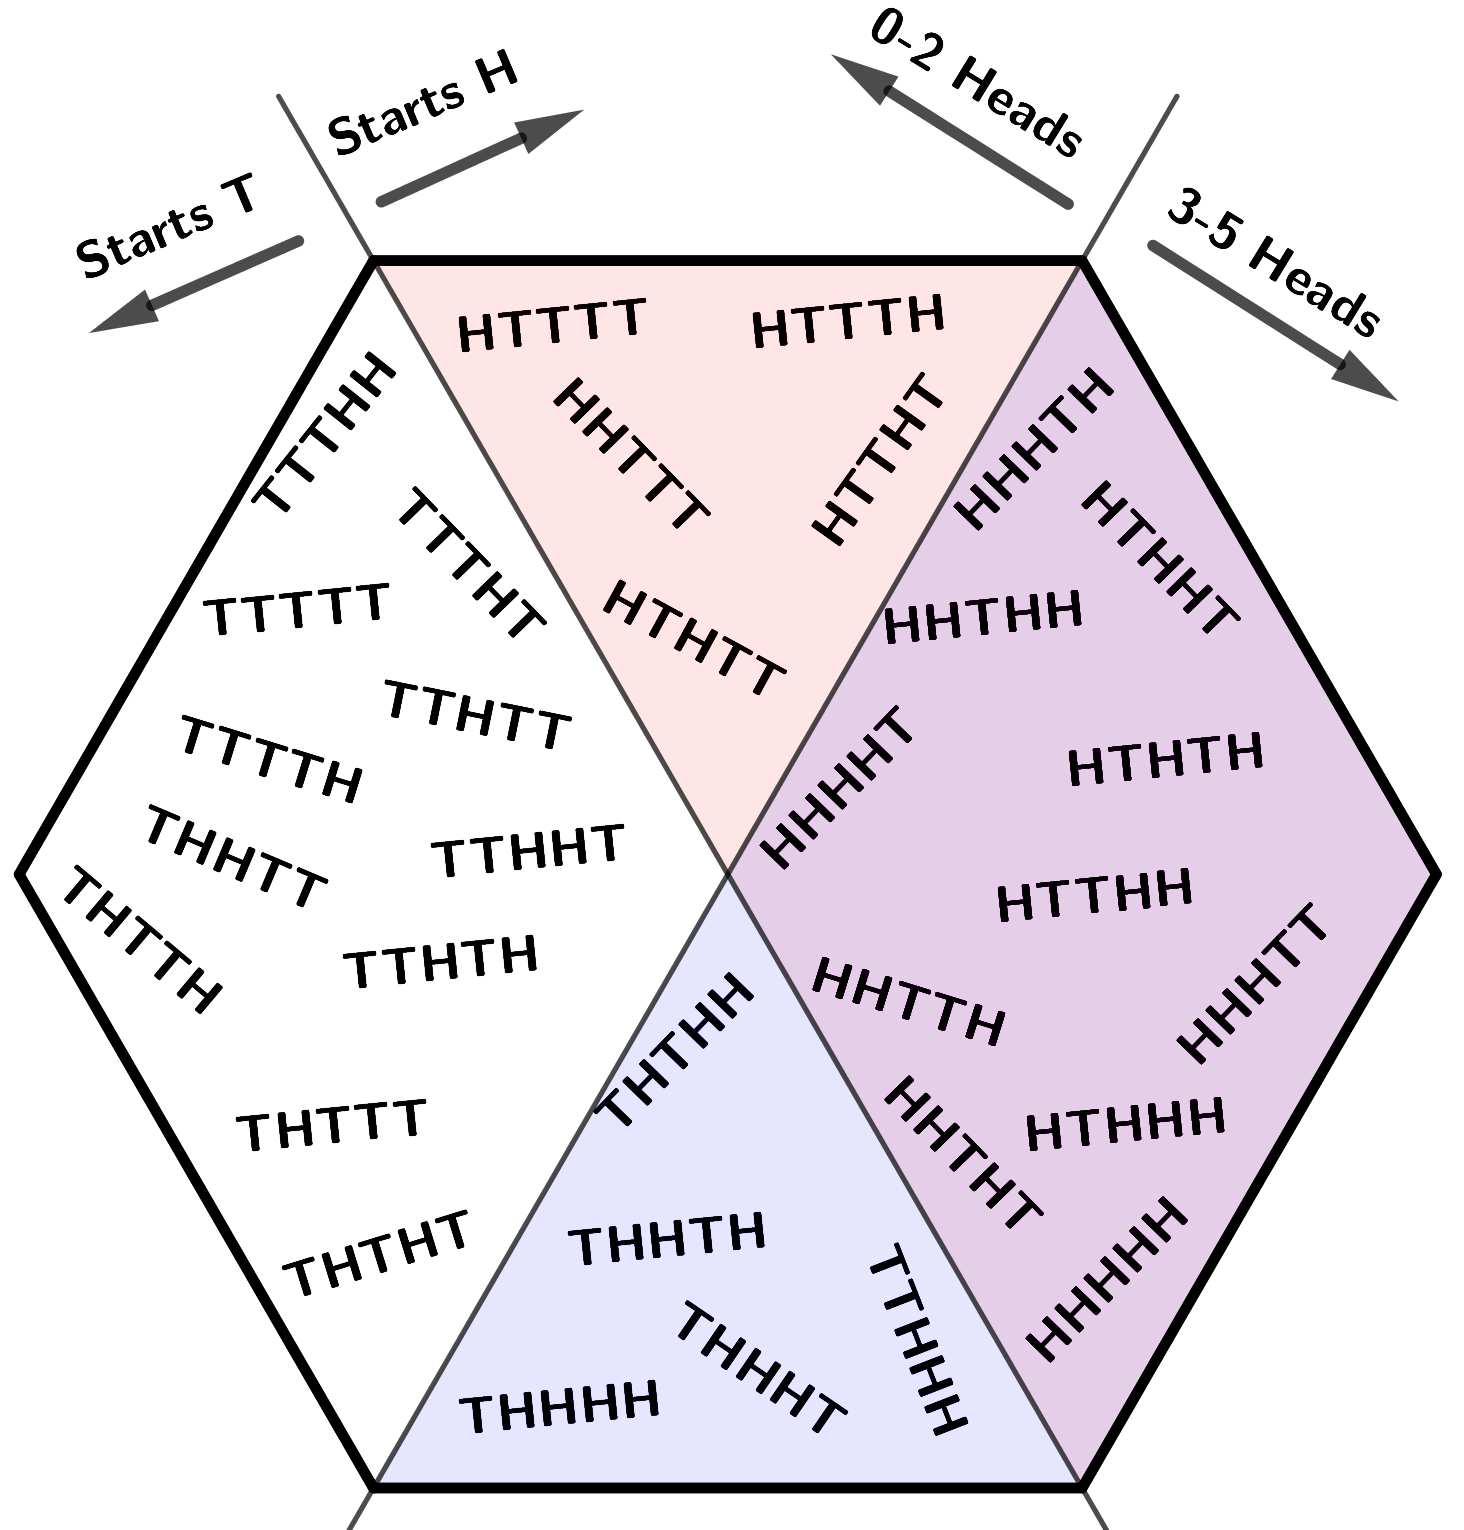
\includegraphics[width=0.52\textwidth]{existing-materials/ProbabilityNotes_23-24/images/condo0.png}\qquad
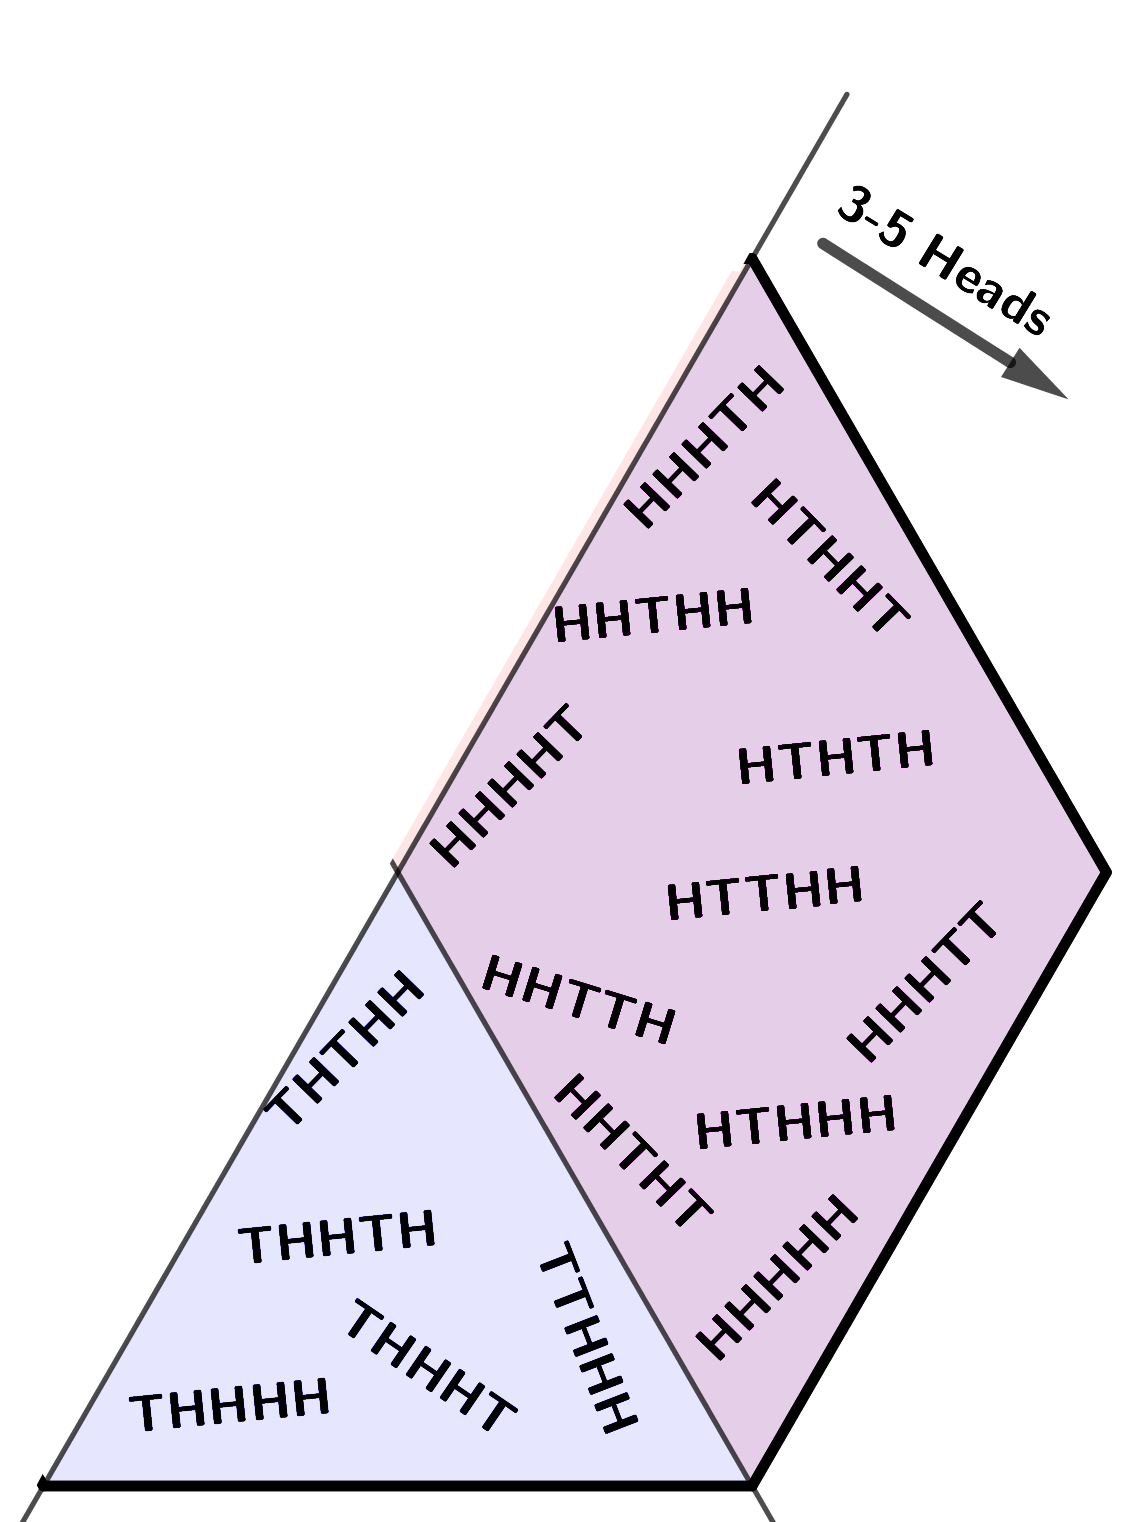
\includegraphics[width=0.4\textwidth]{existing-materials/ProbabilityNotes_23-24/images/condo1.png}
\caption{\label{condo} The whole sample space for 5 coin tosses (left). ``Zooming in'' on the half with $\geq 3$ heads, we see that $11/16$ start with an `H'. So $\PP(\text{starts with H} \st \text{number of H $\geq 3$ }) = 11/16$.} 
\end{figure}

\begin{thm}[\textbf{Bayes' Theorem} ]
Let $A,B$ be events with $\PP(B)\not= 0$. Then 
\[
    \PP( A \st B) = \PP( B \st A) \frac{\PP(A)}{\PP(B)}.
 \]
\end{thm}
\begin{proof}
We compute $\PP(A \cap B)$ in two different ways: 
 \[ 
 \PP(B \st A) \PP(A) = \PP(A \cap B) = \PP(A \st B) \PP(B). 
 \]
Dividing by $\PP(B)$ gives the result. 
\end{proof}
We could easily have solved the problem above using Bayes' Theorem; it would be essentially the same calculation. 
\begin{thm}[\textbf{Bayes' Theorem -  ``probability of causes" form}]
Let our sample space $\Omega$ be partitioned into disjoint events $A_k, \, k=1,2,\dots, n$.  Then for $1\leq j \leq n$, 
\[
   \PP(A_k \st B)  =   \frac{\PP(B \st A_k)\,\PP(A_k)}{ \sum_{i=1}^n \PP(B \st A_i) \,\PP(A_i)}
 \]
\end{thm}
\begin{proof}
Put $A=A_j$ in the previous version of the theorem and then expand $\PP(B)$ using the law of total probability.
\end{proof}

\begin{example}
The use of the the ``probability of causes'' form is more straightforward than it might appear from the statement. 

Tom and Dick are both liars: independently for everything they say, they tell the truth with probability $1/3$ and lie with probability $2/3$.  Tom says something.  Dick tells me that Tom is telling the truth.  What is the probability that Tom is telling the truth? 


\tikzset{
  treenode/.style = {shape=rectangle, rounded corners,
                     draw, align=center,
                     top color=white, bottom color=blue!30},
  root/.style     = {treenode, font=\Large, bottom color=red!30},
  env/.style      = {treenode},
  branch/.style = {treenode, bottom color=blue!10},  
  dummy/.style    = {circle,draw}
}
\tikzstyle{level 1}=[level distance=4.0cm, sibling distance=3.5cm]
\tikzstyle{level 2}=[level distance=5.0cm, sibling distance=2.0cm]

\begin{tikzpicture}
[
grow=right,
    edge from parent/.style = {draw, -latex},
    every node/.style       = {font=\normalsize}
  ]
\node[root]{Tom speaks}
child { 
    node[branch]{Tom lied}
    child { 
        node[env]{Dick says ``Tom told truth''}  
        edge from parent node[above]{$\frac23$} 
        }       
    child { 
        node[env]{Dick says ``Tom lied''}                 
        edge from parent node[above]{$\frac{1}{3}$} 
        }       
    edge from parent node[above]{$\frac23$}            
    }
child { 
    node[branch]{Tom told truth}
    child { 
        node[env]{Dick says ``Tom lied''}                
        edge from parent node[above]{$\frac{2}{3}$} 
        }       
    child { 
        node[env]{Dick says ``Tom told truth''}               
        edge from parent node[above]{$\frac{1}{3}$} 
        }       
    edge from parent node[above]{$\frac{1}{3}$}            
    }     ;           
\end{tikzpicture}

Here, we let $A_1$ be ``Tom told truth'' and let $A_2$ be ``Tom lied''.    We let $B$ be the event that ``Dick says Tom told truth''. 
We are asked to calculate $\PP( A_1 \st B)$. So, using Bayes' theorem in the ``probability of causes'' version we have 
 \begin{eqnarray*}
   \PP( A_1 \st B) &=& 
     \frac{\PP(B \st A_1) \, \PP(A_1)}
     {  \PP(B \st A_1) \,\PP(A_1) + \PP(B \st A_2)\,
         \PP(A_2)   } \\
    &=& \frac{ (1/3)(1/3)}{(1/3)(1/3)+(2/3)(2/3)}  = \frac15. 
 \end{eqnarray*}
\end{example}

\begin{example}
The example we will now study is presented as an ``updating information'' example where we use the original Bayes' theorem.  You might like to convert it to a ``probability of causes'' wording and draw the probability tree to understand the connection.

A suspect X is believed to be guilty of a given crime with probability $\PP(G)=0.6$ on the basis of existing evidence.  The criminal also left a blood stain at the scene. The suspect X has a blood group common to 20\% of the general population.

A test on the blood stain now tells us that it comes from a person with this blood group. How does that affect the probability that the suspect X is guilty? 


Let $B$ be the event that the blood stain has this particular blood group.  We know the blood test will certainly be positive if X is guilty, so $\PP( B \st G) = 1$.  But we want to know the probability of X's guilt, given the new evidence. In other words, we want to find $\PP( G \st B)$. 


First we calculate (law of total probability again) 
 \begin{eqnarray*}
  \PP(B) &=& \PP(\text{X guilty}) \,\PP(B \st \text{X guilty})   + \PP(\text{X not guilty}) \,  \PP(B \st \text{X not guilty} ) \\
  &=& (0.6) (1) + (0.4) (0.2)  = 0.68
 \end{eqnarray*}
 because if X is not guilty, the blood test will be positive with the probability of its being so in the general population.
 
Then according to Bayes' Theorem
 \[
    \PP( G \st B) =  \frac{\PP( B \st G)}{\PP(B)} \, \PP(G)
    =  \frac{1}{0.68} \, 0.6 = 0.88 
 \]
is an updated probability of X's guilt. 

Bayes' Theorem has been widely used in court cases. See \url{https://www.theguardian.com/law/2011/oct/02/formula-justice-bayes-theorem-miscarriage} for a controversy a few years ago around this. (Colin Aitken, until recently in the School of Mathematics in Edinburgh is quoted.) 
\end{example}

\begin{example}
I toss a coin 6 times and get a total of four heads. What is the probability my first roll was heads?  (Ans: $2/3$.) 
\end{example}



\subsection{Exercises} 


\begin{exer}
A very standard example of this sort of ``probability of causes'' analysis is ``false positives'' in medicine. For example, suppose that in the general population, a certain condition is present in 1\% of people.  

There is a test for the condition. The test always returns positive if the subject has the condition.  If the subject does not have the condition, it returns negative 95\% of the time but gives a positive response 5\% of the time.  

A random person takes the test and it returns positive. What is the probability they have the disease? 
\end{exer}

\begin{sol}
You may find drawing the tree helps.   In this case, let $C$ denote the event that the random person has the condition.  Let $T$ denote the event of a positive test result.  From the question 
 \[  
    \PP(C) = 0.01, \quad \PP(C^c) = 0.99, \quad \PP(T \st C) = 1, 
    \quad \PP( T \st C^c)=0.05
 \] 
 where the complement $C^c$ is the event of the person not having the condition. Finally, 
 \[
 \PP(T) = \PP(T \st C) \PP(C) + \PP(T \st C^c) \PP(C^c) = 
   1 (0.01) + 0.05 ( 0.99) = 0.0496.
 \]
We are asked for $\PP( C \st T)$ and so by Bayes,
\[
   \PP(C \st T) = \PP(T \st C) \,\frac{\PP(C)}{\PP(T)} 
   = 1 \; \frac{0.01}{0.0496} = 0.2016. 
\]
(One sees here a basic problem with ``screening'' programmes: unless the test is very reliable, they will throw up many more false alarms than real ones.) 
\end{sol}

\begin{exer}
This sort of information updating with Bayes' Theorem is also an essential ingredient in machine learning. It goes something like this. 

Suppose an image identifying algorithm is trying to decide what sort of animal is appearing in a picture on the web.  The word ``cat'' appears in nearby text so the algorithm's initial hypothesis is it's a cat with probability $0.8$. The algorithm decides that there is a ball of string in the picture. It is known that this is the case for 50\% of cat pictures but also for 10\% of non-cat pictures.  What is the updated probability that the picture shows a cat? 
\end{exer}

\begin{sol}
Here $P(C)0.8$, where $C$ is the event of the picture being of a cat. The probability of a ball of string in the picture is 
 \[
   \PP(S) = \PP(S \st C) \PP(C) + \PP(S \st C^c) \PP(C^c) = 
    0.5 * 0.8 + 0.1 * 0.2 = 0.42,  
 \]
(where $C^c$ is the complement of $C$, i.e.\ the even of the picture not being of a cat).   So, by Bayes: 
 \[
   \PP(C \st S) = \frac{\PP(S \st C)}{\PP(S)} \,\PP(C) =
       \frac{0.5}{0.42} 0.8 = 0.95.
 \]
\end{sol}

\begin{exer}
Tom, Dick and Harry each tell the truth independently with probability $1/3$ and lie with probability $2/3$ every time they speak. Tom says something we don't hear; Dick states whether Tom told the truth or not, but we don't hear that either. Harry says that Dick says that Tom told the truth.  What is the probability that Tom told the truth? 
\end{exer}

\begin{sol}
From a tree, I compute that Harry says that Dick says that Tom told the truth (``HSDSTTT") with probability $13/27$. Also, the conditional probability that Harry says this given that Tom told the truth (``TTT'') is $5/9$. From Bayes (or just analysing the tree),
 \[
   \PP(TTT \st HSDSTTT ) = \PP( HSDSTTT \st TTT) \frac{\PP(TTT)}{\PP(HSDSTTT)} = \frac59 \, \frac{1/3}{13/27} = \frac5{13}. 
 \]
\end{sol}

\subsection{Independence}
\begin{defn}[\textbf{Independence}]
Two events $A,B \subseteq \Omega$ are independent if
\[ \PP(A \cap B) = \PP(A) \PP(B).\]
\end{defn}
\noindent If $\PP(B) \neq 0$ we can re-phrase this as
\[ \PP(A \vert B) = \PP(A),\]
i.e.\ the probability of $A$ happening is the same regardless of whether $B$ happened. \\ \linebreak
\noindent
The event $A \cap B$ is the \emph{intersection} of the two events: it occurs precisely when both $A$ and $B$ occur. We say two events are ``dependent'' if they are not independent. 

We will say more about independence next week.  Two events being independent means that knowing that one has occurred does not change the probability that the other occurs.  

\subsection{Random Variables}

For a binomial distribution problem, the sample space $S$ might be taken to be all the possible $2^n$ length-$n$ sequences of successes and failures. But all we are interested in is the number of successes, which is a function on the sample space taking numerical values.  Thus we make the definition:

\begin{defn}[\textbf{Definition: Random variable}]
A \ul{random variable} is a measurable\footnote{Usually, one has to work hard to construct functions which are not measurable.} function on the sample space.
\end{defn}
Usually, this is $X:\Omega\to \RR$. We usually use capital letters from late in the alphabet (very often $X$) as the symbol for a random variable. 

In probability we will often de-emphasise or even ignore the sample space and work with the random variable directly. 

These capital $X$ random variable gadgets are a bit like the $x$ that appears for a variable in algebra, except that we imagine it takes various different values probabilistically. 

We will assume for now that our random variables, like our sample spaces, are \ul{discrete}; this means that they take a finite or countably infinite number of possible values $x_1, x_2, \dots$.  

\begin{defn}[\textbf{Discrete Uniform random variable}]
We call a random variable $X$ discretely uniformly distributed on $\{ 1, \ldots, n \}$ if
$$ \PP( X =k) = \frac1n \quad \text{for all } k \in \{1,\ldots, n \}.$$
We write
\[X \sim Unif(\{1,\ldots, n\}).\]
\end{defn} 
\noindent Note that we use the symbol `$\sim$' to indicate that a random variable is distributed according to a standard law. 

\begin{defn}[\textbf{Bernoulli random variable}]
A Bernoulli random variable with parameter $p \in [0,1]$ is a random variable such that
\[ \PP(X=1)=p \qquad \text{ and } \qquad \PP(X=0)=1-p=:q. \] 
\end{defn}
\noindent \textbf{Remark:} A Bernoulli random variable is a one-off trial that succeeds with probability $p$.  It is the trivial $n=1$ case of a binomial random variable.

\begin{defn}[\textbf{Binomial random variable}]
A Binomial random variable with parameters $n\in \NN$ and $p \in (0,1)$ is a random variable taking values in $\{0,\ldots,n\}$ with
\[\PP(X=k)= \binom{n}{k} p^k (1-p)^{n-k} = \frac{n!}{k!(n-k)!} p^k (1-p)^{n-k}.\]
We write
\[ X \sim Bin(n,p) \quad \text{or} \quad X \sim Binom(n,p)\]
to indicate that $X$ is distributed as a binomial random variable with parameters $n$ and $p$.
\end{defn}
 
 \ssn{Events}
 When working with a random variable $X$, events can be defined in terms of the values taken.  So for instance $X=3$ and $1 \leq X \leq 4$ define events. Thus we can refer to their probabilities $\PP(X=3)$ and $\PP( 1 \geq X \leq 4)$. 
\end{n}
 
\begin{defn}[\textbf{Definition: Independence of random variables}] 
If we have two random variables $X,Y$ defined on the same sample space we say that $X$ and $Y$ are \ul{independent} if for all values $x,y$ we have 
\[ \PP( \text{$X=x$ and $Y=y$} ) \quad = \quad \PP( X=x) \, \PP(Y=y).\]
\end{defn}
 
\subsection{The Binomial Distribution}

\begin{example}
What is the probability that on rolling three D6 I get exactly one `6'? 

\noindent There are exactly three routes through the tree that give this outcome and each has probability 
 \[
      \left( \frac16 \right) \left( \frac56 \right)^2 = \frac{25}{216}.
 \]
Thus the probability is 
 \[
     3 \frac{25}{216} = \frac{25}{72}. 
 \] 
\end{example}
\noindent \textbf{Generalisation:} Let us consider a general version of the problem.  Supposing we have a process that each time it is carried out produces independently a ``success'' (S) with probability $p$ or a failure (F) with probability $q=1-p$. In the examples in \S\ref{mp2}, success is finding a faulty component or correctly guessing the answer to a question.  We are assuming that each execution of the process is ``independent'', meaning that its success or failure  each time is not influenced by what might have happened before.  If we now repeat this process $n$ times, what is the probability that we get exactly $k$ successes? 
\begin{example}
Suppose $n=10$ and $k=7$ and $p=1/4$. One particular sequence of successes and failures is $SSFFSSFSSS$. Thinking of a large probability tree, the probability of this exact sequence is 
 \[
    ppqqppqppp = p^k q^{n-k} = p^7 q^3 = \left( \frac14 \right)^7 \, \left( \frac34 \right)^3   = \frac{3^3}{4^{10}}
\]
This probability is the same for all the different sequences with seven successes. 

How many other sequences  are there with precisely seven S's?  That is the same question as asking how many ways are there of choosing seven things from ten.  It is the Binomial coefficient
 \[
       \binom{10}7 = \frac{10!}{7! \,3!} = 120. 
  \]
Adding all these possibilities, the probability of three successes in eight trials is exactly 
  \[
     \binom{10}7 p^k q^{n-k} = 120 \frac{3^3}{4^{10}} \approx 0.0031. 
  \]
\end{example}

\begin{exer}
Note that we have just derived the probability of getting exactly 7 out of 10 by guessing in our multiple choice quiz. Work out the probability of getting 8, 9 and 10 out of 10 and hence answer our second motivating problem. 
\end{exer}

\begin{sol}
\[
    \binom{10}{7} \left( \frac13\right)^7 \left( \frac23 \right)^3 +  
    \binom{10}{8} \left( \frac13\right)^8 \left( \frac23 \right)^2 +  
    \binom{10}{9} \left( \frac13\right)^9 \left( \frac23 \right)^1 +  
    \binom{10}{10} \left( \frac13\right)^{10} \left( \frac23 \right)^0  \approx 0.019661636.
 \]
 (I give many decimal places because leaving out the 1/10 possibility only affects the fifth decimal place!) 
\end{sol}

For the general problem, the probability of $k$ successes in $n$ trials is as follows.    
  \[
       \PP( \text{$k$ successes}) =  \binom nk p^k q^{n-k} =  \frac{n!}{k! \, (n-k)!} p^k q^{n-k}. 
  \]

\begin{example}
I roll a D6 twelve times.  How likely is it that I roll precisely two sixes?   Here, $n=12, k=2$ and $p=1/6$. So the answer is 
 \[
    \binom{12}2 \left(\frac{1}{6}\right)^2  \left(\frac{5}{6}\right)^{10}
     \approx 0.296.
 \]
\end{example}

\begin{exer}
I toss a fair coin 6 times.  How likely is it that I roll $k$ heads where $k=0,1,2,3,4,5,6$? 
\end{exer}
\begin{sol}
Use the formula with $n=6$ and $p=1/2$.  For instance, $\PP(k=3) = 20/64 = 5/16$. 
\end{sol}

\begin{table}[h]  
  \begin{tabular}{cc} 
    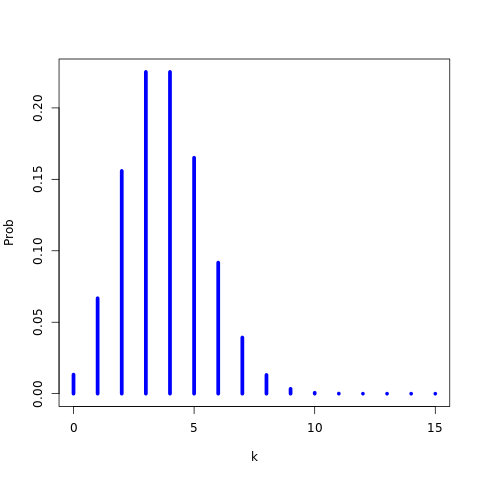
\includegraphics[width=0.45\textwidth]{existing-materials/ProbabilityNotes_23-24/images/binom15P25.png} & 
    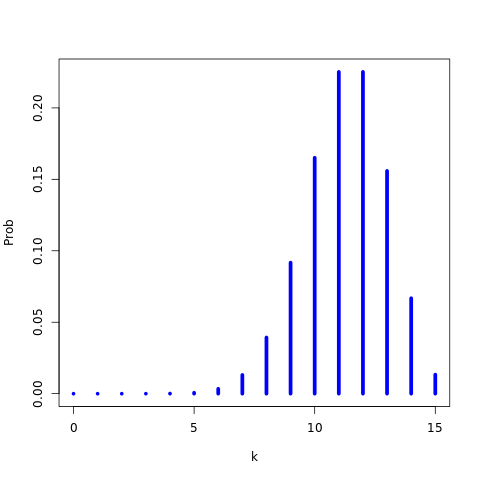
\includegraphics[width=0.45\textwidth]{existing-materials/ProbabilityNotes_23-24/images/binom15P75.png} \\
     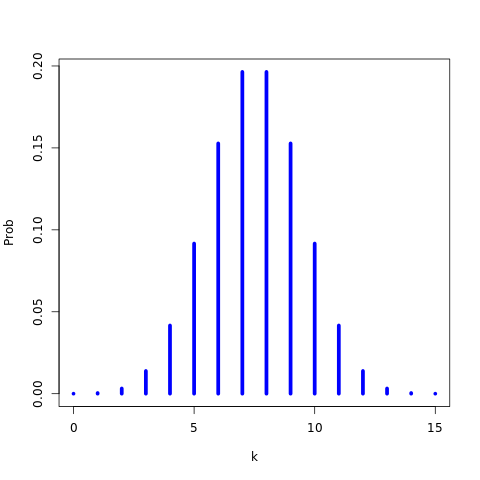
\includegraphics[width=0.45\textwidth]{existing-materials/ProbabilityNotes_23-24/images/binom15P5.png} & 
    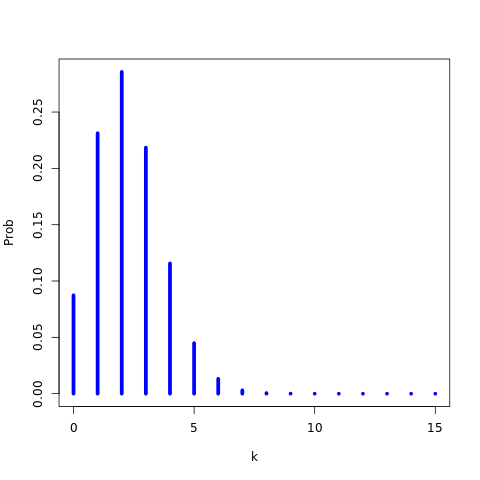
\includegraphics[width=0.45\textwidth]{existing-materials/ProbabilityNotes_23-24/images/binom15P15.png} \\
  \end{tabular}
 \caption{\label{binpics} Binomial with $n=15$ and $p=0.15, 0.25, 0.5, 0.75$ in some order}
\end{table}


\sse
In table~\ref{binpics} ``probability mass functions'' for Binomial distributions with different probabilities are plotted. The height of each vertical bar is the probability of the corresponding outcome. Which is which?
\end{e}

\sss
The top row has $p=0.25$ and $p=0.75$. Note the symmetry between them. 
The bottom two are $p=0.5$ (note the symmetry about its centre) and $p=0.15$. 
\end{s}

\sse{}
\begin{enumerate}
    \item 
Compute the `Red v Blue' and `Green v Red' probabilities with a tree.
 \item Compute the win probability of Blue versus Green where the game is to roll two blue dice versus two green dice with the higher total winning. 
\end{enumerate}
Answers to these can be found in the Workshop 1 solutions. 
\end{e}

